\chapter{指数函数和对数函数}
1.指数与对数\\
指数法则:\\
(1)任意非零数的零次幂是1. 表示为:\quad$b^0=1$\\
(2)一个数的一次幂刚好是该数本身. 表示为:\quad$b^1=b$\\
(3)将两个底数相同的幂相乘时, 将指数相加. 表示为:\quad$b^xb^y=b^{x+y}$\\
(4)将两个底数相同的幂相除时, 将分子的指数减去分母的指数. 表示为:\quad$\displaystyle\frac{b^x}{b^y}=b^{x-y}$\\
(5)取幂的幂时, 将指数相乘. 表示为:\quad$(b^x)^y=b^{xy}$\\

.对数法则:\\
(1)1的对数是0. 表示为:\quad$\log_b(1)=0$\\
(2)任意正数以该数本身为底的对数是1. 表示为:\quad$\log_b(b)=1$\\
(3)乘积的对数是对数的和. 表示为:\quad$\log_b(xy)=\log_b(x)+\log_b(y)$\\
(4)商的对数是对数的差. 表示为:\quad$\displaystyle\log_b(\frac{x}{y})=\log_b(x)-\log_b(y)$\\
(5)一个数的幂的对数是指数倍该数的对数. 表示为:\quad$\log_b(x^y)=y\log_b(x)$\\
(6)一个数的幂为底的对数是指数的倒数倍该数为底的对数. 表示为:\quad$\displaystyle\log_{b^n}x=\frac{1}{n}\log_bx$\\
(7)\quad 换底法则:对于任意的底数$b>1$和$c>1$及任意的$x>1$
\[\log_b(x)=\frac{\log_c(x)}{\log_c(b)}\]
注: 对数的底取值范围: $(0,1)\bigcup(1,\infty)$\\[2ex]

2.$e$的定义\\
$e$的取值\\
\[e=2.718\quad281\quad828\quad459\quad045\quad\ldots\]

底数为$e$的对数称为\textbf{自然对数}\\[2ex]

3.指数与对数的极限\\
\begin{center}
	\framebox{$\displaystyle\lim_{n\to\infty}(1+\frac{x}{n})^n=e^x$}
\end{center}
\begin{center}
\framebox{$\displaystyle\lim_{n\to\infty}(1+\frac{1}{n})^n=e$}
\end{center}
例1.
\phantom{例}$\displaystyle\lim_{x\to 0}(1+h^2)^{\frac{1}{3h^2}}$\\
推导过程:\\
$\displaystyle\lim_{x\to 0}(1+h^2)^{\frac{1}{3h^2}}=\lim_{x\to 0}[(1+h^2)\frac{1}{h^2}]^{\frac{1}{3}}=e^{\frac{1}{3}}$\\

例2.\\
\phantom{例}$\displaystyle\lim_{x\to\infty}\frac{2x^2+3x-1}{e^{\frac{1}{x}}(x^2-7)}$\\
推导过程:\\
$\displaystyle\lim_{x\to\infty}\frac{2x^2+3x-1}{e^{\frac{1}{x}}(x^2-7)}=\lim_{x\to\infty}\frac{1}{e^{\frac{1}{x}}}\frac{2x^2+3x-7}{x^-7}=1\times2=2$\\

\begin{center}
		\framebox{$\displaystyle\lim_{x\to\infty}\frac{x^n}{e^x}=0$}
\end{center}
例.\\
\phantom{例}$\displaystyle\lim_{x\to\infty}\frac{x^8+100x^7-4}{e^x}$\\
推导过程:\\
当$x\to\infty$时, $\displaystyle\frac{x^8+100x^7-4}{}\backsim\frac{x^8}{e^x}$\\
$\displaystyle\lim_{x\to\infty}\frac{x^8+100x^7-4}{e^x}=\lim_{x\to\infty}\frac{x^8}{e^x}=0$\\

\begin{center}
		\framebox{$\displaystyle\lim_{x\to\infty}\frac{\ln x}{x^a}=0$, 其中$a>0$}
\end{center}
例.\\
\phantom{例}$\displaystyle\lim_{x\to\infty}\frac{\log_7(x^3+3x-1)}{x^{0.1}-99}$\\
推导过程:\\
当$x\to\infty$时, $\displaystyle x^3+3x-1\backsim x^3$, $\displaystyle x^{0.1}-99\backsim x^{0.1}$\\
$\displaystyle\lim_{x\to\infty}\frac{\log_7(x^3+3x-1)}{x^{0.1}-99}=\lim_{x\to\infty}\frac{\log_7x^3}{x^{0.1}}=0$\\

\begin{center}
		\framebox{$\displaystyle\lim_{x\to 0^+}x^a\ln(x)=0$, 其中$a>0$}
\end{center}

4.对数和指数求导
\begin{center}
		\framebox{$\displaystyle\frac{\dif }{\dif x}\log_b(x)=\frac{1}{x\ln(b)}$}
\end{center}
\begin{center}
		\framebox{$\displaystyle\frac{\dif }{\dif x}\ln(x)=\frac{1}{x}$}
\end{center}
\begin{center}
		\framebox{$\displaystyle\frac{\dif }{\dif x}(b^x)=b^x\ln(b)$}
\end{center}
\begin{center}
		\framebox{$\displaystyle\frac{\dif }{\dif x}(e^x)=e^x$}
\end{center}

5.取对数求导法\\
假设
\[y=f(x)^{g(x)}\]
关于$y$的求导步骤, 如下:\\
1)等式两边取自然对数, 得:
\[\ln(y)=g(x)\ln(f(x))\]
2)等式两边关于$x$作隐式求导, 得:
\[\frac{1}{y}\frac{\dif y}{\dif x}=g'(x)\ln f(x)+\frac{f'(x)}{f(x)}g(x)\]
3)等式两边乘以$y$, 再将$y$替换为$f(x)^{g(x)}$, 得:
\[\frac{\dif y}{\dif x}=[g'(x)\ln(f(x))+\frac{f'(x)}{f(x)}g(x)]f(x)^{g(x)}\]

例1.
\phantom{例}$\displaystyle\frac{\dif}{\dif x}(x^{\sin(x)})$\\
推导过程:\\
$\displaystyle y=x^{\sin(x)}$\\
1)等式两边取自然对数:\\
\phantom{\qquad}$\displaystyle\ln(y)=\sin(x)\ln(x)$\\
2)等式两边关于$x$隐式求导:\\
\phantom{\qquad}$\displaystyle\frac{1}{y}\frac{\dif y}{\dif x}=\cos(x)\ln(x)+\frac{\sin(x)}{x}$\\
3)等式两边乘以$y$, 并将$y$替换为$x^{\sin(x)}$:\\
\phantom{\qquad}$\displaystyle\frac{\dif y}{\dif x}=\left[\cos(x)\ln(x)+\frac{\sin(x)}{x}\right]x^{\sin(x)}$\\[1ex]

例2.\\
\phantom{例}$\displaystyle\frac{\dif}{\dif x}[(1+x^2)^{\frac{1}{x^3}}]$\\
推导过程:\\
$\displaystyle y=(1+x^2)^{\frac{1}{x^3}}$\\
1)等式两边取自然对数:\\
\phantom{\qquad}$\displaystyle\ln(y)=\frac{1}{x^3}\ln(1+x^2)$\\
2)等式两边关于$x$隐式求导:\\
\phantom{\qquad}$\displaystyle\frac{1}{y}\frac{\dif y}{\dif x}=-\frac{3}{x^4}\ln(1+x^2)+\frac{2x}{x^3(1+x^2)}=\frac{2}{x^2(1+x^2)}-\frac{3\ln(1+x^2)}{x^4}$\\
3)等式两边乘以$y$, 并将$y$替换为$(1+x^2)^{\frac{1}{x^3}}$:\\
\phantom{\qquad}$\displaystyle\frac{\dif y}{\dif x}=\left[\frac{2}{x^2(1+x^2)}-\frac{3\ln(1+x^2)}{x^4}\right](1+x^2)^{\frac{1}{x^3}}$\\[2ex]

6.指数增长与指数衰变\\
(1)指数增长方程: $\displaystyle P(t)=P_0e^{kt}$\\
例.\\
\phantom{空格}假如三年前兔子的总数是1000只, 而现在增长至64000只, 那么从现在开始, 一年后兔子总数是多少?\\
解答:\\
由指数增长方程:\\
\phantom{\qquad}$\displaystyle 64000=1000e^{3k}$\\
\phantom{\qquad}$\displaystyle k=\frac{\ln64}{3}=2\ln2$\\
一年后兔子总量:\\
$\displaystyle P(4)=1000e^{8\ln2}=1000\times2^8=256000$\\[1ex]

(2)指数衰变方程: $P(t)=P_0e^{-kt}$\\
例.\\
\phantom{空格}如果原料的半衰期为七年, 开始时有50磅原料, 十年后还剩多少磅? 多久之后, 原料会减少到1磅?\\
解答:\\
由指数衰减方程:\\
\phantom{\qquad}$\displaystyle P(7)=\frac{1}{2}P_0=P_0e^{-kt}$\\
\phantom{\qquad}$\displaystyle k=\frac{\ln2}{7}$\\
十年之后剩余的磅数:\\
$\displaystyle P(10)=P_0e^{-kt}=50e^{-\frac{10ln2}{7}}$\\
原料剩余1磅所需要的时间:\\
$\displaystyle P(t)=50e^{-\frac{\ln2}{7}t}=1$\\
$\displaystyle\frac{\ln2}{7}t=\ln50$\\
$\displaystyle\phantom{\frac{\ln2}{7}}t=\frac{7\ln50}{\ln2}$\\[2ex]

7.双曲函数\\
(2)双曲正弦: $\displaystyle\sinh(x)=\frac{e^x-e^{-x}}{2}$\\[1ex]
如图:
\begin{figure}[H]
\centering
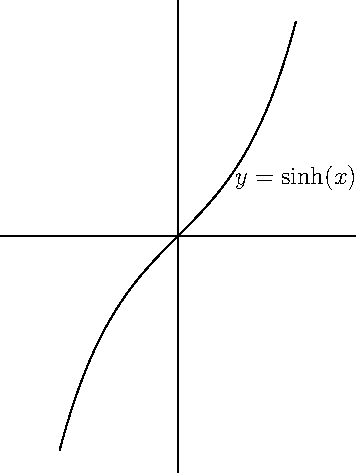
\includegraphics{sinh.pdf}
\end{figure}
(2)双曲余弦: $\displaystyle\cosh(x)=\frac{e^x+e^{-x}}{2}$\\[1ex]
如图:
\begin{figure}[H]
\centering
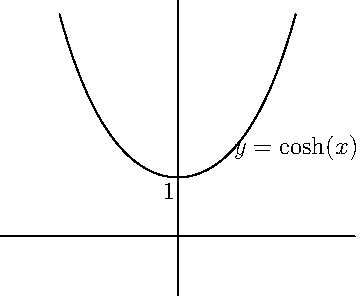
\includegraphics{cosh.pdf}
\end{figure}
(3)双曲线方程: $\cosh^2(x)-\sinh^2(x)=1$\\[1ex]

%最后编辑于: 2022-01-21
